\documentclass[a4paper, 11pt]{article}
\usepackage[utf8]{inputenc}
\usepackage[left=2cm,text={17cm, 24cm},top=3cm]{geometry}
\usepackage[czech]{babel}
\usepackage[T1]{fontenc}
\usepackage[unicode]{hyperref}
\usepackage{times}
\usepackage{csquotes}
\usepackage{graphicx}
\usepackage{amssymb}
\usepackage{amsmath}
\usepackage{amsthm}
\usepackage{multirow}
\graphicspath{ {./images/} }
\usepackage[noline,czech,ruled,longend,linesnumbered, vlined]{algorithm2e}
\usepackage{pdflscape}
\usepackage{tikz}
\usepackage{collcell}

\title{IMP}
\author{Simona Češková (xcesko00)}
\date{\today}


\begin{document}
\begin{titlepage}
\begin{center}
\Huge
\textsc{Vysoké učení technické v~Brně\\
\huge{Fakulta informačních technologií}} \\
\vspace{\stretch{0.382}}
\LARGE
Mikroprocesorové a vestavěné systémy \\
\Huge{M - ESP32: Přístupový terminál} \\
\vspace{\stretch{0.618}}
\end{center}
{\Large \today \hfill Simona Češková (xcesko00)}\\
\end{titlepage}
\tableofcontents
\newpage

\section{Úvod do problému}
\subsection{ESP32}
Mikroprocesor ESP32, konkrétně wemos d1 r32 je deska s integrovaným WiFi modulem s čipem ESP-32. Obsahuje USB rozhraní pro jeho programování i napájení. Komunikaci zajišťuje řadič CH340. ESP-32 je 32 bitovým mikroprocesorem a GPIO piny, které mohou vykonávat činnost podle naprogramovaného kódu. \href{https://www.laskakit.cz/wemos-d1-r32-uno-esp32/}{[1]}

Mikroprocesory jsou zařížení, která slouží k více účelům a dají se naprogramovat, díky tomu, že na vstupu akceptují digitální data, je poté dokážou spracovat a z nich zobrazit výstup, který zobrazuje výsledek. Spracování je díky instrukcím, které mají uložené v paměti.\href{https://www.giga-pc.cz/slovnik-pojmu/procesor/}{[2]}

\subsubsection{Input a output rozhraní}
Pro spuštění programu je nutné mít na mikroprocesor ESP32 připojenou klávesnici 3x4 a 2 LED diody. To znamená, že z ESP32 bude využito 9 input/output portů + port GND. 

\subsection{Použité knihovny}
\begin{itemize}
    \item freertos/FreeRTOS.h - práce s edf prostředím
    \item freertos/task.h - vytváření tasků - souběžně probíhajících procesů
    \item freertos/queue.h - využívání čekání
    \item driver/gpio.h - nastavování pinů - obsahuje většinu použitých funkcí
\end{itemize}

\subsection{Použité rozhraní}
Program byly spoušteň a překládán pomocí aplikace ESP-IDF 5.0 CMD a tudíž napsán v nejnovější verzi 5.0.

\subsection{Zapojení pinů z 3x4 klávesnice do ESP32}
Na obrázků níze jsou zaznačeny modrou barvu čísla pinů, které se nachází na klávesnici. Tyto piny jsou zapojeny do GIO portů na ESP32, jejichž číslo je označeno barvou zelenou.

\begin{figure}[h]
    \centering
    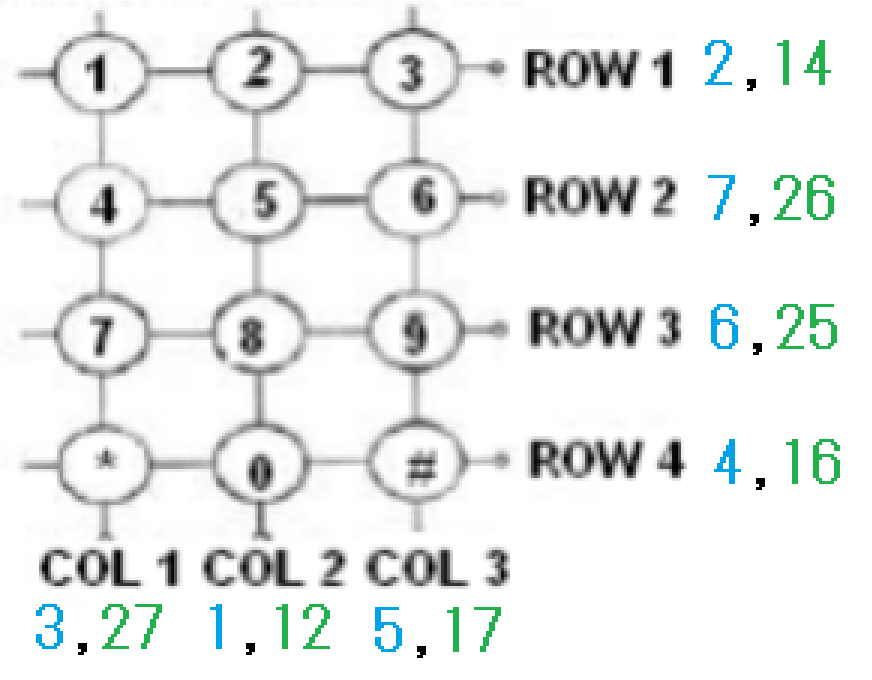
\includegraphics[width=0.45\textwidth]{pins.png}
    \caption{Rozložení pinů na klávesnici}
    \label{fig:pins.png}
\end{figure}
 Dvě LED diody - červená a zelená - jsou zapojeny v tomto pořadí do GIOP 13 a GIOP 5. Pro ně je dále nutné k nim přidat rezistor, který bude mezi Vcc a anodou. Katoda bude vést do GND.
Pro správný chod programu je nutné takto mikro procesor s klávesnicí a diodami zapojit.

\newpage

\section{Popis řešení}
\subsection{Rozdělení na podproblémy při řešení}
\subsubsection{Detekce stisknutého tlačítka}
Detekce tlačítla funguje tak, že se do řádků a nebo sloupců postupně pouští Vcc napětí a kontroluje se, zda do konkrétního tlačítla (kombinace jednoho sloupce a jednoho řádku) se napětí dostalo. V případě řešení mého projektu jsem zvolila procházení přes sloupce. Do prvního sloupce nastavím pomocí funkce \verb!gpio_set_level()! \verb!OUTPUT! level na 1 (\verb!high!). Protože jsou všechny sloupce nastaveny díky \verb!gpio_set_direction()! na \verb!OUTPUT!, tak v tomto momentě srkze něj může procházet napětí. Poté je nutné zkontrolovat, zda prvním řádkem prošlo napětí - port, který odpovídá danému řádku, bude mít nastavený level na 1. To lze zjistit pomocí funkce \verb!gpio_get_level()!. Pokud ano, tak kombinace sloupce a řádku odpovídá stisknutému tlačítku, jinak se zkontrolují zbyté tři řádky. Na konci toho úseku kontroly se nastaví level sloupce zpět na 0 pomocí \verb!gpio_set_level()!, aby se tento proces mohl zopakovat pro další sloupec.

\subsubsection{Použití přerušení}
Přerušení je ansynchroní operací, při které procesor přeruší vykonávanou instrukci, obslouží zdroj vyvolaného přerušení a poté pokračuje v plnění dalších instrukcí. Zdroj přerušení je jakákoliv změna, která se stane během běhu programu. Během obsluhy přerušení není možné provádět jiné změny, než ty které obsahuje, proto je to bezpečná cesta pro provádění změn. U nastavení řádků \verb!gpio_cfg.intr_type! je použila typ \verb!GPIO_INTR_POSEDGE!, který značí \verb!rising edge!, proto při kontrole řádků se kontroluje zda je jeho level nastaven v 1. V ten moment se zvedá hrana napětí a vyvolá se přerušení.

\subsubsection{Zkombinování ověřování na klávesnici s prací s LED diodami}
Při výkonu nějaké činnosti ve nějaké funkci, v které je třeba iniciovat změnu stavu diody a jejího svícení, se zavolá daná funkce z hlavního \verb!while! cyklu. V tomto případě nejde o žádné složité výpočty, proto není třeba používat druhého procesu, který by obsluhoval zároveň diody a práci s heslem.

\subsubsection{Použití funkce \texttt{vTaskDelay()}}
Tato funkce slouží k vyvování zpoždění/počkání a je nutné ji použít za čáct kódu v kterých se nastavují důležité změny, aby se nestalo, že program pojede v procesu dál, ale změny se stihnou zapsat až za běhu.

\subsection{Kostra programu}
\subsubsection{Inicializace portů a proměnných}
První sekci programu tvoří funkce pro inicializaci:
\begin{itemize}
    \item \verb!disable_interrupt()! vypne možnost dostávat přerušení, protože se nachází v přerušení.\\ \verb!Enable_interrupt()! jej zase zapne.
    \item \verb!init_ports()! - nastaví porty 
    \begin{itemize}
        \item nejdříve vyresetuje porty a jejich původní nastavení pomocí funkce \verb!gpio_reset_pin()!
        \item pomocí struktury \verb!gpio_config_t!, na kterou jsem přišla díky demu cvičení v přednášce "Platforma ESP32 a její programování" na stránce Elearning. tato struktura umožňuje nastavit pro více portů vlastnosti současně. Po nastavení všech parametrů se konfigurace díky funkci \verb!gpio_config! uloží do registrů.
        \item nastaví řádům \verb!pulldown! registry funkcí a zároveň vypne \verb!gpio_pullup! registry, aby nedošlo k případným chybám.
        \item jako poslední přiředí portům správnou funkci. Všechny sloupce jsou pouze v \verb!OUTPUT! módu, protože z nich napětí může pouze odcházet dál a naopak všechny řádky jsou v \verb!INPUT! módu, protože u nich chceme zpětnou vazbu, jestli jimi teče napětí. Diody jsou stejně jako sloupce v \verb!OUTPUT! módu.
    \end{itemize}
    \item \verb!init_gpio()! jsem taktéž použila díky demo cvičení. Nejprve povolí přerušení pro všechny sloupce, poté vytvoří \verb!xQueueCreate!, která je dále volaná ve \verb!while_loop()! funkci jako \verb!xQueueReceive!. Ta čeká až přijde nějaký požadavek, jakmile se tak stane, tak vrátí \verb!TRUE! a program se v tomto případě dostane dál k testování jaké tlačítko na klávesnici bylo zmáčknuto. Mimo toho ještě nastavuje pomocí \verb!gpio_isr_handler_add()! \verb!ISR handler! = obsluhu přerušení pro odpovídající GPIO piny.
\end{itemize}
\subsubsection{Hlavní běh programu}
\begin{itemize}
    \item \verb!while_loop()! označuje cyklus v kterém se nekonečně dokola kontroluje, jestli nebyla nějaká klávesa zmáčknutá.
\end{itemize}

\subsubsection{Funkce pro práci s diodami}
\begin{itemize}
    \item díky \verb!led_flash()! zabliká dioda, protože obsahuje funkci \verb!gpio_set_level!, která nastaví pomocí globálních proměnných (\verb!R_LED_state! a \verb!G_LED_state!) diodám 1 pro svícení, nebo 0 pro zhasnutí.
    \item \verb!good_G_LED()! pro signalizaci, že bylo heslo zadáno správně
    \item \verb!wrong_R_LED()! pro situaci, při které bylo zle zadáno heslo
    \item \verb!both_LED()! umožňuje uživateli viděť kdy zadal správně heslo při pokusu o změnu hesla. V tomto módu se čeká až zadá nové heslo. Poté se uloží.
\end{itemize}
    
\subsubsection{Pomocné funkce pro ověřování hesel}
\begin{itemize}
    \item \verb!compare()! porovnává uložené heslo s nově zadaným heslem
    \item \verb!add_char()! přidá znak do proměnného pole, dokud nedojde k poslednímu ze čtyř znaků a poté je díky \verb!compare()! porovná.
    \item \verb!store_new_password()! uloží nové heslo do pole \verb!code_array!, v kterém se uchová
    \item \verb!before_changing_password()! kontrola jestli bylo správně zadné původní heslo, pro púmožnění jeho změny na nové
\end{itemize}

\newpage
\section{Zhodnocení}
\subsection{Úskalí řešení projektu}
Nejtěžší na projektu bylo na začátku správně nastavit prostředí pro běh programu. Měla jsem problém jak s instalací rozšíření Platformia a IDF do Visual Studio Code, tak i s instalací konzole .\href{https://dl.espressif.com/dl/esp-idf/}{ESP-IDF pro Windows}. Naštěstí se to později podařilo a již poté se psal projekt dobře. 

\subsection{Ověření vlastností řešení}
Pro ověření správné činnosti je nutné se podívat na problém i jako uživatel a podle toho vytvořit prostředí, které bude především uživatelsky přívětivé. Uživatel očekává zpětnou vazbu, které mu dodávají v tomto případě pouze LED diody. Proto je vhodné zpětně signalizovat podařené i nepodařené úspěchy přihlášení takovou cestou, kterou by uživatel jako chování čekal. Červená LED dioda slouží pro negativní signalizaci, zelená LED dioda pro positivní signalizaci a pokud jsou obě použity zároveň, tak uživatel tuší, že došlo k speciálnímu stavu (vybrání nového hesla). Pro použití v reálném životě by bylo lepší vzhledem k bezpečnosti využít možnost zhasnutí obou LED diod, aby signalizace nepřilákala pozornost okolí. Pro účely jasné zpěné vazby v tomto projektu jsem ponechala signalizaci za použití obou LED diod.

\subsection{Výsledek}
Výsledkem projektu je program pro mikrokontroler ESP32, který dokáže zpracovávat data, která dostal pomocí externí klávesnice. Zpracováním se myslí ošetření neplatných vstupů. U platných vstupů podle jejich sekvence určit zda se jedná o požadované heslo, nebo ne a podle toho se zachovat. Umožňuje i změnu hesel i když vždy po restartování u sobě nechá uložené základní heslo (1234).

\subsection{Možné rozšíření}
K řešení by se daly přidat i další inovace, například podpora více znakového hesla, dále povolení využít maximálně $n$ pokusů ($n \in \mathbb{N}$) do zablokování a následné odblokování jednotným speciálním kódem.

\newpage

\renewcommand{\refname}{Literatura}
\bibliographystyle{czechiso}
\bibliography{IMS}
\end{document}
